\documentclass{cubeamer}
\usepackage{listings}

\title{How to \LaTeX: a (too) short introduction}
\subtitle{Journal Club}
\author[Janek Gr\"ohl]{Janek Gr\"ohl}
\date{\today} % or whatever the date you are presenting in is
\institute[University of Cambridge]{Cancer Research UK Cambridge Institute, University of Cambridge\\
Department of Physics, University of Cambridge}
% \copyrightnotice{Published by the American Institute of Aeronautics and Astronautics, Inc., with permission}

\begin{document}

\maketitle

\cutoc

\section{What is \LaTeX?}

\begin{frame}{It's pronounced "$\Lambda\alpha\theta\epsilon\chi$".}
\begin{minipage}{0.45\textwidth}
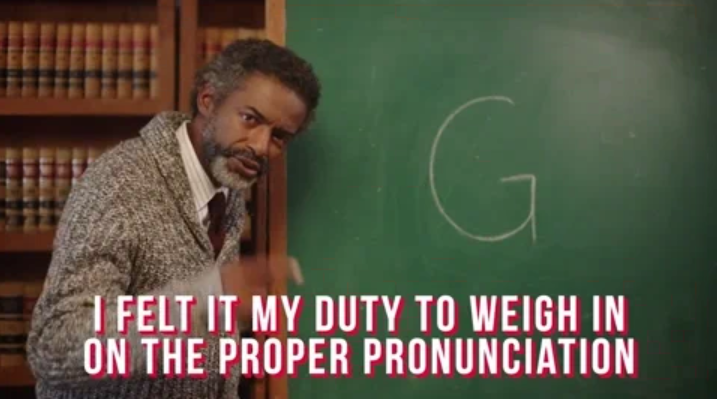
\includegraphics[width=0.9\textwidth]{img/pronunciation.png}
\end{minipage}
\begin{minipage}{0.5\textwidth}
    \textit{Insiders pronounce the χ of TeX as a Greek chi, not as an ‘x’, so that TeX rhymes with the word blecchhh. It’s the ‘ch’ sound in Scottish words like loch or German words like ach; it’s a Spanish ‘j’ and a Russian ‘kh’. \textbf{\color{red} When you say it correctly to your computer, the terminal may become slightly moist.}} \cite{knuth1984texbook}
\end{minipage}
\end{frame}

\begin{frame}{Separation of Content from Style}
\begin{minipage}{0.45\textwidth}
Content:\\
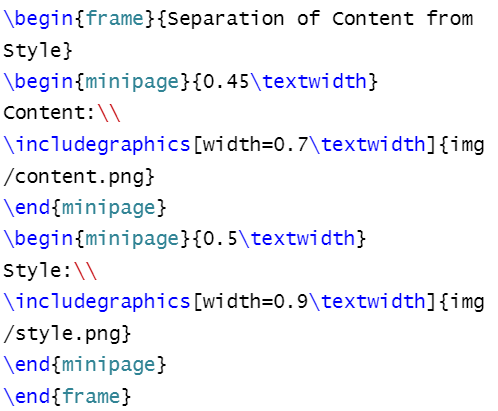
\includegraphics[width=0.7\textwidth]{img/content.png}
\end{minipage}
\begin{minipage}{0.5\textwidth}
Style:\\
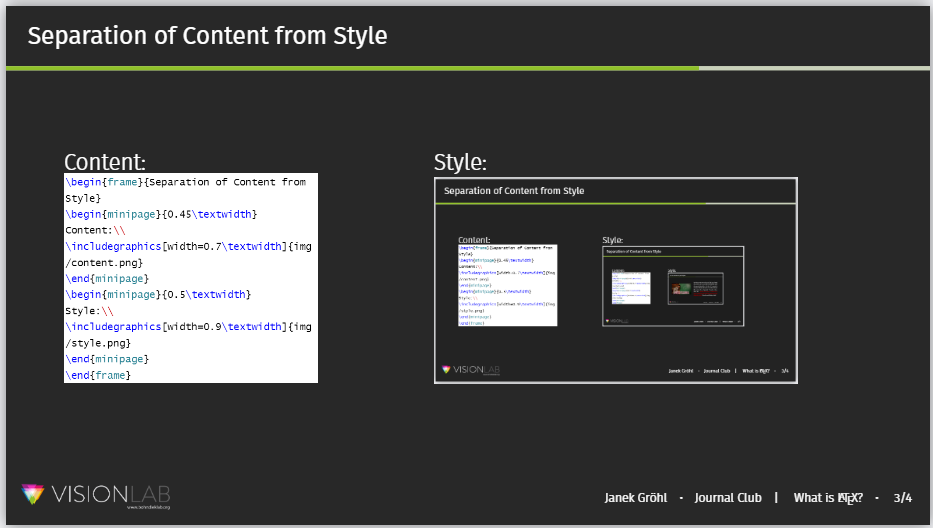
\includegraphics[width=0.9\textwidth]{img/style.png}
\end{minipage}
\end{frame}

\begin{frame}[fragile]{Minimal example for LaTeX document structure}

\begin{verbatim}
    \documentclass[12pt,a4paper]{article}
    \begin{document}
        \title{Title}   \author{Name}   \date{\today}
        
        \maketitle
        
        \section{First section}
        \subsection{Subsection}
        \section{Second section}
        
        \bibliography{bibliography_file.bib}
    \end{document}
\end{verbatim}

\end{frame}

\section{When might it be wise to use it?}

\subsection{Large documents}

\subsection{Math notation}

\subsection{Bibliography management}

\subsection{Extensibility}

\section{Why doesn't everyone use it??}

\subsection{Learning Curve}

\subsection{Counterintuitivity}

\subsection{Setting it up on a local computer}

\section{A practical guide to \LaTeX}

\subsection{Overleaf}

\subsection{Some handy commands}

\begin{frame}[fragile]{Document Structure Commands}
    \begin{tabular}{lll}
         \textbf{Command} &	\textbf{Level} &	\textbf{Comment}\\
         \\
         \hline
        \verb+\part{''part''}+ & -1 &not in letters\\
        \verb+\chapter{''chapter''}+ & 0 & only books and reports\\
        \verb+\section{''section''}+ &	1 &	not in letters\\
        \verb+\subsection{''subsection''}+ & 2 & not in letters\\
        \verb+\subsubsection{''subsubsection''}+ & 3 & not in letters\\
        \verb+\paragraph{''paragraph''}+ & 4 & not in letters\\
        \verb+\subparagraph{''subparagraph''}+ & 5 & not in letters\\
        \hline
    \end{tabular}
\end{frame}

\begin{frame}[fragile]{Document Structure Commands (without explicit numbering)}
    \begin{tabular}{lll}
         \textbf{Command} &	\textbf{Level} &	\textbf{Comment}\\
         \\
         \hline
        \verb+\part*{''part''}+ & -1 &not in letters\\
        \verb+\chapter*{''chapter''}+ & 0 & only books and reports\\
        \verb+\section*{''section''}+ &	1 &	not in letters\\
        \verb+\subsection*{''subsection''}+ & 2 & not in letters\\
        \verb+\subsubsection*{''subsubsection''}+ & 3 & not in letters\\
        \verb+\paragraph*{''paragraph''}+ & 4 & not in letters\\
        \verb+\subparagraph*{''subparagraph''}+ & 5 & not in letters\\
        \hline
    \end{tabular}
\end{frame}


% \begin{frame}{Frame Title}
%     \begin{itemize}
%         \item Use
%         \item Figures,
%         \item Do
%         \item Not
%         \item Use
%         \item Bullet
%         \item Points
%     \end{itemize}
% \end{frame}

% \begin{frame}{Use meaningful titles that actually provide information}
%     \begin{columns}
%         \begin{column}{0.6\textwidth}
%             \begin{figure}
%                 \centering
%                 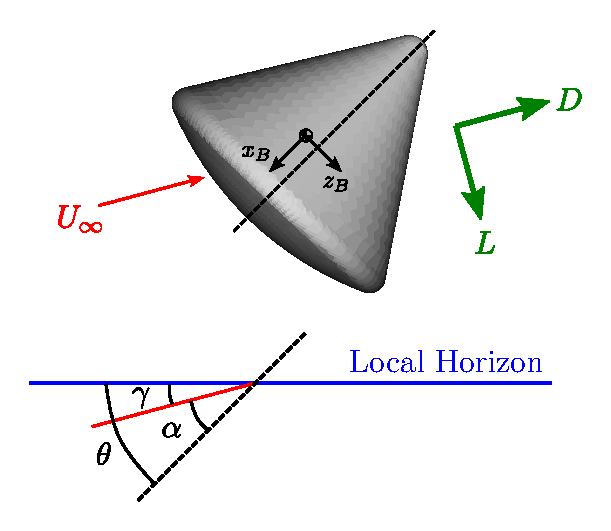
\includegraphics[height = 0.7\textheight]{img/example.pdf}
%                 \caption{Fancy Thing from \textit{Source et al.}}
%             \end{figure}
%         \end{column}
%         \begin{column}{0.4\textwidth}
%             \begin{itemize}
%                 \item Some
%                 \item Interesting
%                 \item Points
%             \end{itemize}
%         \end{column}
%     \end{columns}
% \end{frame}

% \section{A Section}

% \begin{frame}{Make your presentation interactive}
%     \begin{cublock}[What about a question to the audience?]
%         \begin{overlayarea}{\textwidth}{\baselineskip}
%             \only<2->{Followed by the answer.}
%         \end{overlayarea}
%     \end{cublock}
% \end{frame}

% % Q&A
% \begin{frame}
%     \Huge\textsc{Thank You}
    
%     \vfill
    
%     \LARGE\textsc{Questions?}
% \end{frame}

% \appendix

% \begin{frame}{Backup slides go here}
    
% \end{frame}

\begin{frame}{Bibliography}
\bibliographystyle{apalike}
\bibliography{bibliography.bib}
\end{frame}

\end{document}
